\subsection{Functions defined almost everywhere}

In conformity with the definition in No.~3, a mapping f of a subset A of X into a set F is said to be defined almost everywhere if the complement of the set A on which it is defined is a negligible set. We again call equivalence class of f, and denote by \(\widetilde{f}\) , the equivalence class of every function defined on all of X and equal to \(f(x)\) at the points \(x \in X\) where f is defined; it is clear that this class depends only on f.~Two functions f, g defined almost everywhere are again said to be equivalent if \(\widetilde{f} = \widetilde{g}\) : this means, therefore, that the set of points where \(f(x)\) and \(g(x)\) are both defined and equal has negligible complement.

It follows at once that Prop. 8 of No.~4 and its corollary may be generalized to the case where in their statements it is assumed only that each of the functions \(f_{n}, g_{n}\) is defined almost everywhere; then the functions \(\varphi((f_{n}))\)

and \(\varphi((g_n))\) are themselves defined almost everywhere; the equivalence class of \(\varphi((f_n))\) is again \(\varphi((\widetilde{f}_n))\) .

A function defined almost everywhere, with values in a vector space F, is again said to be negligible if it is equivalent to 0. If f is a negligible function with values in F, and u is a linear mapping of F into a vector space G, then the composite function \(u \circ f\) (defined almost everywhere) is negligible; similarly, for every (finite) numerical function g, defined almost everywhere, the function gf (defined almost everywhere) is negligible.

\pandocbounded{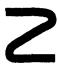
\includegraphics[keepaspectratio]{images/part001_e94daaaa.jpg}}

One must take care to observe that, in the set of functions with values in F and defined almost everywhere, the internal law of composition \((\mathbf{f},\mathbf{g})\mapsto\mathbf{f}+\mathbf{g}\) is not a group law, because, while the function 0 is indeed a neutral element for this law, if f is not everywhere defined then there does not exist a function g such that \(f+g=0\) . This is what motivates the introduction of the equivalence classes \(\widetilde{f}\) , which do form a vector space.

Let \((f_n)\) be a sequence of mappings into a topological space F, each of which is defined almost everywhere in X. We say that the sequence \((f_n)\) converges (pointwise) almost everywhere to f in X if the set of points \(x \in X\) where all the \(f_n(x)\) are defined and the sequence \((f_n(x))\) has a limit equal to \(f(x)\) , has negligible complement. It is clear that if, for each n, the function \(g_n\) (defined almost everywhere) is equivalent to \(f_n\) , then the sequence \((g_n)\) converges almost everywhere to f.

If F is topological vector space, one defines similarly an almost everywhere convergent series, whose general term is a function \(f_{n}\) defined almost everywhere in X with values in F; the sum of this series is a function defined at the points where the partial sums \(\sum_{k=1}^{n}\mathbf{f}_{k}(x)\) are defined and have a limit, and its class depends only on the classes \(\widetilde{f}_{n}\) .

